%!TEX root = ../thesis.tex

\chapter{Theoretical motivation}
\label{chap:motivation}
%!TEX root = ../../thesis.tex


\section{The Standard Model of particle physics}
	\label{sec:sm}
	%!TEX root = ../../thesis.tex

The \ac{SM} of particle physics is a gauge quantum field theory describing the kinematics and interactions of sub-atomic particles \cite{Aitchison,Peskin}. The dynamics of such a 
theory are determined by the symmetries respected by the Lagrangian density.
The \ac{SM} is invariant under local transformations of the \SMgroup gauge group,
resulting in the strong, weak and electromagnetic forces of nature and determining
the particle content of the theory. Additionally, invariance under global 
transformations of the Poincaré group ensures the theory is identical in all 
inertial frames of reference, as asserted by special relativity.

Each gauge theory of the \ac{SM} describes the dynamics of a force of nature, which 
is mediated by a number of gauge bosons and couples to a conserved current, in 
accordance with Noether's theorem. \ac{QCD} describes the strong 
interaction, is mediated by eight gluons and couples to colour charge. \ac{QED}
describes the electromagnetic interaction, is mediated by the 
photon and couples to electric charge. The weak interaction is mediated by the massive 
\PWpm and \PZ bosons and is understood within the context of \ac{EW} theory,
a unification of the electromagnetic and weak interactions. A quantum field theory of
gravity is not included in the \ac{SM}. It is important to note that the gauge groups of 
the strong and weak interactions are non-abelian. Physically, this means that the
gauge bosons are themselves charged and therefore experience self-interactions.

\begin{figure}
	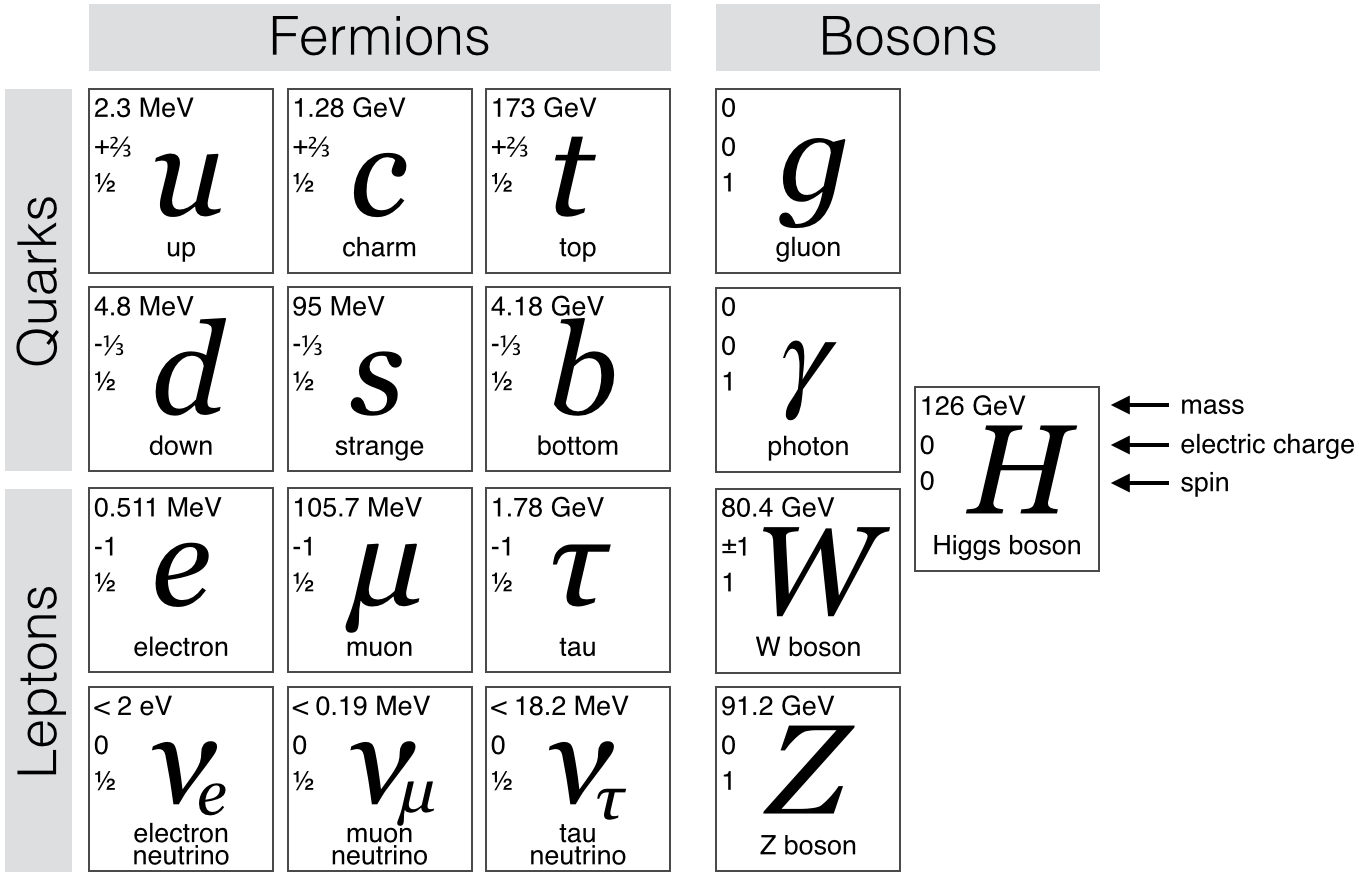
\includegraphics[width=\largefigwidth]{tex/motivation/sm_particles}
	\caption{The particle content of the \ac{SM}. Particle masses from \cite{PDG}.
	\todo[inline]{Should I remove the Higgs mass here?}}
	\label{fig:sm_particles}
\end{figure}

The elementary particles of the \ac{SM} are summarised in \Figure~\ref{fig:sm_particles}.
They are naturally separated into bosons (integer spin) and fermions (half-integer spin).
In addition to the gauge bosons previously introduced, the Higgs boson is a by-product
of electroweak symmetry breaking (described in \Section~\ref{sec:ewsb}) and its
couplings are proportional to mass. The twelve flavours of fermions are categorised 
according to the interactions they experience, or equivalently the charges they posses: 
quarks (strong, electromagnetic, weak), charged leptons (electromagnetic, weak) and 
neutrinos (weak). The fermions are also arranged in three generations of increasing
mass - the first generation are stable since they cannot decay to lower mass particles.
Most particles have an associated antiparticle with identical mass but inverted internal 
quantum numbers.

\section{Electroweak unification}
	\label{sec:ewsb}
	%!TEX root = ../../thesis.tex

The first theory of weak interactions was a four-point interaction with Fermi coupling 
constant \unit{$G_{\text{F}} = 1.166\times 10^{-5}$}{\GeV\rpsquared}. Although successful 
in describing low energy phenomena, such as nuclear $\beta$-decay and muon decay, at 
energies above \unit{\about300}{\GeV} the theory predicted cross sections which violate 
unitarity \cite{Aitchison}.

The solution was to introduce charged vector bosons (\PWpm bosons) to mediate the weak 
interaction, similar to the exchange of photons in \ac{QED}. However, unlike \ac{QED}, 
the weak interaction is short ranged and therefore its exchange bosons must be massive. 
Since the propagator for a particle of mass $m$ and momentum $p$ contains a factor 
$1 / (p^2 - m^2)$, in the low energy limit we can relate to Fermi's theory and identify
\begin{equation}
	G_{\text{F}} \sim g^2 / m_{\PW}^2
\end{equation}
where $g$ is the coupling of the vector boson. Thus, at low energies, the strength of the 
weak interaction is suppressed by the mass of the exchange boson.

At this time, there were two key obstacles to unifying the electromagnetic and weak 
interactions. First, the discovery of parity violation in cobalt-60 $\beta$-decay 
implied the weak interaction has a \VminusA structure, whereas \ac{QED} has a pure V 
structure \cite{Wu:1957}.\footnote{
	Five bilinear covariants can be constructed from the Dirac $\gamma$ matrices, which 
	are named according to how they transform under parity: scalar, pseudoscalar, vector, 
	axial vector and tensor.
}
Second, the \PWpm bosons are massive whilst photons are massless. This was a major 
problem because gauge bosons are inherently massless.\footnote{
	Consider the gauge transformation of a Yang-Mills gauge field 
	$\bvec{W}_{\mu} \rightarrow \bvec{W}_{\mu} - \partial_{\mu} \bvec{\alpha}(x)
	- g \lbrack \bvec{\alpha}(x) \times \bvec{W}_{\mu} \rbrack$. Clearly the mass term 
	$-\tfrac{1}{2}m^2 \bvec{W}_{\mu} \cdot \bvec{W}^{\mu}$ is not gauge invariant, and 
	hence the gauge boson is massless.}
In fact, fermion masses were also forbidden by the chiral nature of the weak interaction, 
but were known to exist.\footnote{
	Consider a spinor as the sum of its left- and right-handed chiral states 
	$\psi = \psi_{\text{L}} + \psi_{\text{R}}$. Then the Dirac mass term is 
	$-m \bar{\psi} \psi = -m (\bar{\psi}_{\text{R}} \psi_{\text{L}} + 
	\bar{\psi}_{\text{L}} \psi_{\text{R}})$. For a chiral theory, $\psi_{\text{L}}$ and
	$\psi_{\text{R}}$ behave differently under gauge transformations and thus the mass 
	term is not gauge invariant.
}

Glashow's proposal of an \EWgroup group was a major step forward \cite{Glashow:1961}. 
This model describes three gauge fields \rowthreevec{W^1_{\mu}}{W^2_{\mu}}{W^3_{\mu}} 
which couple to weak isospin $T$ with strength $g$, and a single gauge field $B_{\mu}$ 
which couples to weak hypercharge $Y$ with strength $g'$. The subscript L indicates 
that only left-handed chiral particles couple to the $W^i_{\mu}$ fields, explaining the 
\VminusA nature of the weak interaction whilst preserving \ac{QED}. The physical gauge 
fields are obtained through the mixing of these fields
\begin{align}
	W^{\pm}_{\mu} &= (W^1_{\mu} \mp i W^2_{\mu}) / \sqrt{2} \label{eq:Wfield} \\
	Z_{\mu} &= \cos\thetaW W^3_{\mu} - \sin\thetaW B_{\mu} \label{eq:Zfield} \\
	A_{\mu} &= \sin\thetaW W^3_{\mu} + \cos\thetaW B_{\mu} \label{eq:Afield}
\end{align}
where
\begin{equation}
	\cos\thetaW = g/\sqrt{g^2 + g'^2}
	\quad\quad \text{and} \quad\quad
	\sin\thetaW = g'/\sqrt{g^2 + g'^2} \,. 
	\label{eq:weak_mixing}
\end{equation}
We identify $W^{\pm}_{\mu}$ with the \PWpm bosons, $A_{\mu}$ with the photon 
and $Z_{\mu}$ with a new neutral \PZ boson. Weak neutral currents were later confirmed 
experimentally \cite{Gargamelle:1973}. 

Glashow's \EWgroup theory therefore predicts the interaction of fermions, in left-handed 
\SUgroup{2} doublets and right-handed \SUgroup{2} singlets (see 
\Table~\ref{tab:ew_fermions}), with \PWpm, \PZ and \Pphoton 
exchange bosons. Gauge boson self-interactions are also expected due to the non-abelian 
nature of the \ac{EW} theory. The \PWpm bosons couple to weak isospin $T$ with strength 
$g$, the \PZ boson couples vectorially to $c_{\text{V}}$ and axially to $c_{\text{A}}$ 
with strength $g/(2\cos\thetaW)$, and the photon couples to electric charge $Q$ with 
strength $e = g\sin\thetaW$, where
\begin{align}
	c_{\text{V}} &= T_3 - 2 Q \sin^2\thetaW \,,\quad\quad c_{\text{A}} = T_3 \\
	Q   &= T_3 + \frac{Y}{2} \,.
\end{align}

\begin{table}[b]
	\begin{tabular}{ccc@{\hskip 1cm}cccc}
		\toprule
		& & & $T$ & $T_3$ & $Y$ & $Q$ \\
		\midrule
		\multirow{2}{*}{$\colvector{\Pnue\\ \Pe}_{\!\!\!\text{L}}$} & 
		\multirow{2}{*}{$\colvector{\Pnum\\ \Pmu}_{\!\!\!\text{L}}$} & 
		\multirow{2}{*}{$\colvector{\Pnut\\ \Ptau}_{\!\!\!\text{L}}$} & 
		$\tfrac{1}{2}$ & $+\tfrac{1}{2}$ & $-1$ & 0 \\
		& & & $\tfrac{1}{2}$ & $-\tfrac{1}{2}$ & $-1$ & $-1$ \\
		$\Pnue_{\text{R}}$ & $\Pnum_{\text{R}}$ & $\Pnut_{\text{R}}$ & 0 & 0 & 0 & 0 \\
		$\Pe_{\text{R}}$ & $\Pmu_{\text{R}}$ & $\Ptau_{\text{R}}$ & 0 & 0 & $-2$ & $-1$ \\
		\midrule
		\multirow{2}{*}{$\colvector{\Pup\\ \Pdown'}_{\!\!\!\text{L}}$} & 
		\multirow{2}{*}{$\colvector{\Pcharm\\ \Pstrange'}_{\!\!\!\text{L}}$} & 
		\multirow{2}{*}{$\colvector{\Ptop\\ \Pbottom'}_{\!\!\!\text{L}}$} & 
		$\tfrac{1}{2}$ & $+\tfrac{1}{2}$ & $+\tfrac{1}{3}$ & $+\tfrac{2}{3}$ \\
		& & & $\tfrac{1}{2}$ & $-\tfrac{1}{2}$ & $+\tfrac{1}{3}$ & $-\tfrac{1}{3}$ \\
		$\Pup_{\text{R}}$ & $\Pcharm_{\text{R}}$ & $\Ptop_{\text{R}}$ & 0 & 0 & $+\tfrac{4}{3}$ & $+\tfrac{2}{3}$ \\
		$\Pdown_{\text{R}}$ & $\Pstrange_{\text{R}}$ & $\Pbottom_{\text{R}}$ & 0 & 0 & $-\tfrac{2}{3}$ & $-\tfrac{1}{3}$ \\
		\bottomrule
	\end{tabular}
	\caption{The weak isospin $T$, weak hypercharge $Y$ and electric charge $Q$ of the 
	fermions. In charged currents, the states that couple to \Pup-type 
	quarks are superpositions of \Pdown-type quarks and are denoted with a prime. 
	Although right-handed neutrinos are decoupled, recent observations of neutrino 
	oscillations suggest these might exist.}
	\label{tab:ew_fermions}
\end{table}

Unfortunately, it was necessary to explicitly break the symmetry by adding mass terms for 
the \PWpm and \PZ bosons by hand. Initial attempts to invoke a mechanism of \ac{SSB} were 
hindered by the Goldstone theorem.



\subsection{The Goldstone theorem}
\label{sec:ewsb:goldstone}
\ac{SSB} arises when the vacuum state does not respect the symmetry in question. This can 
occur when a field acquires a non-zero vacuum expectation value. To see this, consider a 
complex scalar field $\phi$ described by the Lagrangian
\begin{equation}
	\mathcal{L} 
	= \parenths{\partial_{\mu}\phi^{\dagger}} \parenths{\partial^{\mu}\phi} 
	+ \mu^2 \phi^{\dagger}\phi - \lambda \parenths{\phi^{\dagger}\phi}^2
	\label{eq:lagr:goldstone}
\end{equation}
with positive $\mu^2$ and $\lambda$, giving a sombrero potential 
(\Figure~\ref{fig:sombrero}). 
Although $\mathcal{L}$ is invariant under global \Ugroup{1} transformations 
$\phi \rightarrow \eexp{-i\alpha} \phi$, there are infinite degenerate vacua
$\phi = \mu\eexp{-i\theta}/\sqrt{2\lambda}$ that are not invariant. In order to interact 
with the system, a single vacuum must be arbitrarily chosen, spontaneously breaking the 
\Ugroup{1} symmetry.

\begin{figure}[b]
	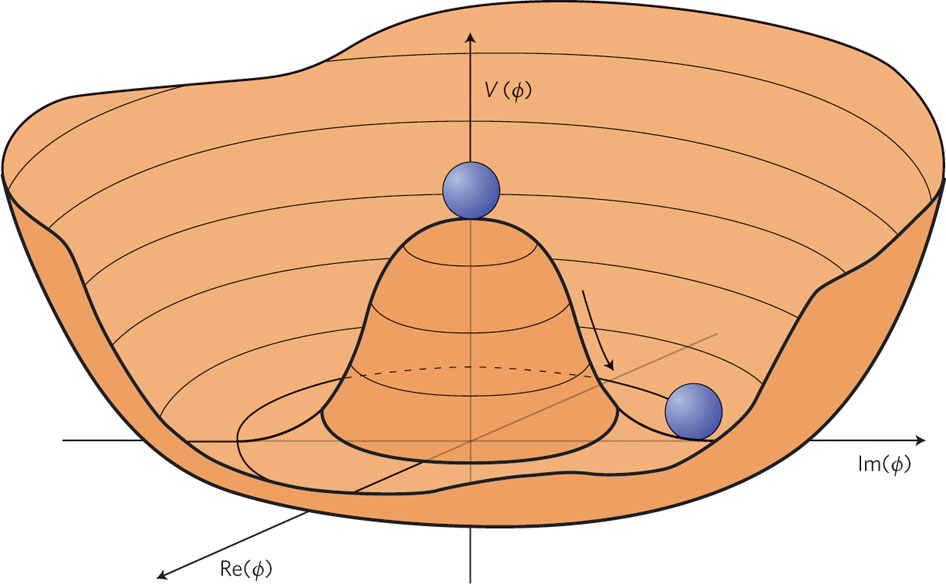
\includegraphics[width=\mediumfigwidth]{tex/motivation/sombrero}
	\caption{The sombrero potential, in which a vacuum state must be arbitrarily chosen, 
	spontaneously breaking the symmetry of the underlying Lagrangian.
	Fluctuations in the azimuthal direction correspond to a massless Nambu-Goldstone 
	boson. Fluctuations in the radial direction correspond to a massive Higgs boson.}
	\label{fig:sombrero}
\end{figure}

The Goldstone theorem states that \ac{SSB} of a continuous global symmetry will lead to 
the existence of a number of massless scalar Nambu-Goldstone bosons \cite{Goldstone:1962}.
This can be seen by considering radial and azimuthal excitations, $h\parenths{x}$ and 
$\theta\parenths{x}$, about the vacuum 
\begin{equation}
	\phi\parenths{x} = \frac{1}{\sqrt{2}} \sqbracs{v + h\parenths{x}} \eexp{-i\theta\parenths{x} / v}
\end{equation}
where $v = \mu/\sqrt{\lambda}$. When substituted into (\ref{eq:lagr:goldstone}), we get
\begin{equation}
	\mathcal{L} = \tfrac{1}{2}\partial_{\mu}\theta \partial^{\mu}\theta
	+ \tfrac{1}{2}\partial_{\mu}h \partial^{\mu}h
	- \mu^2 h^2
	+ \dots
\end{equation}
where the dots denote terms neither kinetic nor mass. 
We identify a massless Nambu-Goldstone boson (the $\theta$-mode) and a Higgs boson of 
mass $\sqrt{2}\mu$ (the $h$-mode).

In order to explain massive \PWpm and \PZ bosons, the electroweak symmetry must be broken.
But the Goldstone theorem suggested that this would predict massless scalar bosons, which
were not experimentally observed.



\subsection{The Higgs mechanism}
\label{sec:ewsb:higgs}
However, when \ac{SSB} of a continuous \textit{local} symmetry is studied, something 
remarkable happens. The Nambu-Goldstone bosons of the theory are `eaten' by the gauge 
bosons, giving them mass. The associated degrees of freedom appear as longitudinal 
components of the massive gauge bosons. This is known as the Higgs mechanism 
\cite{Englert:1964,Higgs:1964a,Higgs:1964b,Guralnik:1964,Higgs:1966}.

Consider the Lagrangian for a \Ugroup{1} gauge theory with a sombrero potential
\begin{equation}
	\mathcal{L} 
	= \parenths{D_{\mu}\phi}^{\dagger} \parenths{D^{\mu}\phi}
	- \tfrac{1}{4} F_{\mu\nu} F^{\mu\nu}
	+ \mu^2 \phi^{\dagger} \phi - \lambda \parenths{\phi^{\dagger} \phi}^2
	\label{eq:lagr:abelHiggs}
\end{equation}
where $D_{\mu} = \partial_{\mu} + iqA_{\mu}$ is the covariant derivative and $F_{\mu\nu} 
= \partial_{\mu}A_{\nu} - \partial_{\nu}A_{\mu}$ is the field tensor. This is invariant 
under local \Ugroup{1} transformations $\phi \rightarrow \eexp{-i\alpha\parenths{x}} \phi$
when accompanied by a gauge transformation of the potential 
$A_{\mu} \rightarrow A_{\mu} + \tfrac{1}{q}\partial_{\mu} \alpha\parenths{x}$.

We are free to choose the unitary gauge $\alpha\parenths{x} = -\theta\parenths{x}/v$,
absorbing the $\theta$-mode into the photon field 
$A_{\mu} \rightarrow A_{\mu} - \tfrac{1}{qv}\partial_{\mu} \theta\parenths{x}$. 
Ultimately, the final result is gauge-independent, but other choices require the 
Nambu-Goldstone bosons to be explicitly included in the Feynman rules. Since the 
$\theta$-mode is `gauged away', excitations about the vacuum become
\begin{equation}
	\phi\parenths{x} = \frac{1}{\sqrt{2}} \sqbracs{v + h\parenths{x}}
\end{equation}
and the Lagrangian (\ref{eq:lagr:abelHiggs}) becomes
\begin{equation}
	\mathcal{L}
	= \tfrac{1}{2} q^2 v^2 A_{\mu} A^{\mu}
	- \tfrac{1}{4} F_{\mu\nu}F^{\mu\nu}
	+ \tfrac{1}{2} \partial_{\mu}h \partial^{\mu}h
	- \mu^2 h^2
	+ \dots
\end{equation}
where the dots denote terms neither kinetic nor mass. 
The Nambu-Goldstone boson is no longer present and the photon has acquired a mass $qv$.
Again, there is a massive scalar Higgs boson as a by-product of the \ac{SSB}.



\subsection{Glashow-Salam-Weinberg electroweak theory}
The Higgs mechanism can be extended to non-abelian gauge theories, as was necessary to 
describe electroweak symmetry breaking \cite{Kibble:1967,Weinberg:1967,Salam:1968}.
Consider the Lagrangian for an \SUgroup{2}\cross\Ugroup{1} gauge theory with a sombrero
potential
\begin{equation}
	\mathcal{L} 
	= \parenths{D_{\mu}\phi}^{\dagger} \parenths{D^{\mu}\phi}
	- \tfrac{1}{4} \bvec{F}_{\mu\nu} \cdot \bvec{F}^{\mu\nu}
	- \tfrac{1}{4} G_{\mu\nu} G^{\mu\nu}
	+ \mu^2 \phi^{\dagger} \phi - \lambda \parenths{\phi^{\dagger} \phi}^2
	\label{eq:lagr:ewHiggs}
\end{equation}
where $D_{\mu} = \partial_{\mu} + \tfrac{i}{2} g \bvec{\tau} \cdot \bvec{W}_{\mu} + 
\tfrac{i}{2} g' Y B_{\mu}$ is the covariant derivative, and $\bvec{F}_{\mu\nu} = 
\partial_{\mu}\bvec{W}_{\nu} - \partial_{\nu}\bvec{W}_{\mu} - g \bvec{W}_{\mu} \cross 
\bvec{W}_{\nu}$ and $G_{\mu\nu} = \partial_{\mu}B_{\nu} - \partial_{\nu}B_{\mu}$ are the
field tensors. In this case, $\phi$ is an \SUgroup{2} doublet of complex scalar fields
\begin{equation}
	\phi = \colvector{\phi^+\\\phi^0} = \frac{1}{\sqrt{2}} \colvector{ \phi_1 + i\phi_2\\ \phi_3 + i\phi_4}.
\end{equation}

Again, there are infinite degenerate vacua satisfying 
$\parenths{\phi_1^2 + \phi_2^2 + \phi_3^2 + \phi_4^2} = \mu^2/\lambda$. In analogue with 
the abelian Higgs mechanism, the unitary gauge absorbs the $\phi_1$, $\phi_2$ and 
$\phi_4$-modes into the gauge fields. Thus, considering excitations about the vacuum
\begin{equation}
	\phi\parenths{x} = \frac{1}{\sqrt{2}} \colvector{0\\  
	v + h\parenths{x}} \label{eq:higgs_doublet}
\end{equation}
the Lagrangian (\ref{eq:lagr:ewHiggs}) becomes
\begin{align}
	\mathcal{L} &= \tfrac{1}{8} g^2 v^2 \bvec{W}_{\mu} \cdot \bvec{W}^{\mu} - \tfrac{1}{4} \bvec{F}_{\mu\nu} \cdot \bvec{F}^{\mu\nu} + \tfrac{1}{8} v^2 g'^2 B_{\mu} B^{\mu} - \tfrac{1}{4} v^2 gg' B_{\mu} W_{3}^{\mu} - \tfrac{1}{4} G_{\mu\nu} G^{\mu\nu} \nonumber \\
	&\quad\quad {} + \tfrac{1}{2} \partial_{\mu}h \partial^{\mu}h - \mu^2 h^2 + \dots \\
	&= \tfrac{1}{4} g^2 v^2 W^{+}_{\mu} W^{-\mu} - \tfrac{1}{2} \parenths{\partial_{\mu}W^{+}_{\nu} - \partial_{\nu}W^{+}_{\mu}} \parenths{\partial^{\mu}W^{-\nu} - \partial^{\nu}W^{-\mu}} \nonumber \\
	&\quad\quad {} + \tfrac{1}{8} v^2 \parenths{g^2 + g'^2} Z_{\mu} Z^{\mu} - \tfrac{1}{4} \parenths{\partial_{\mu}Z_{\nu} - \partial_{\nu}Z_{\mu}} \parenths{\partial^{\mu}Z^{\nu} - \partial^{\nu}Z^{\mu}} - \tfrac{1}{4} F_{\mu\nu} F^{\mu\nu} \nonumber \\
	&\quad\quad {} + \tfrac{1}{2} \partial_{\mu}h \partial^{\mu}h - \mu^2 h^2 + \dots
\end{align}
where the dots denote terms neither kinetic nor mass, $F_{\mu\nu}$ is the field tensor of
\ac{QED}, and the expression has been rewritten in terms of the physical gauge fields 
using (\ref{eq:Wfield}), (\ref{eq:Zfield}) and (\ref{eq:Afield}). The \PWpm bosons 
acquire a mass $gv/2$ and the \PZ boson acquires a mass $v \sqrt{\parenths{g^2+g'^2}}/2$, 
while the photon is massless. Again, all Nambu-Goldstone bosons are gone and a Higgs 
boson has appeared as a by-product of the \ac{SSB}.

This theory predicts a striking relation between the gauge boson masses, using 
(\ref{eq:weak_mixing})
\begin{equation}
	\mW = \mZ \cos\thetaW
\end{equation}
which was experimentally verified once the \PW and \PZ bosons were discovered 
\cite{UA1:Wboson,UA2:Wboson,UA1:Zboson,UA2:Zboson,UA1:1989}. It also predicted a massive 
scalar Higgs boson, whose mass could not be determined from the other parameters of the 
theory.

Fermion masses can also be incorporated into \ac{EW} theory through Yukawa couplings.
Consider a coupling between the electron-type \SUgroup{2} doublet (see 
\Table~\ref{tab:ew_fermions}), the Higgs doublet $\phi$ given in 
(\ref{eq:higgs_doublet}), and the electron \SUgroup{2} singlet
\begin{align}
	\mathcal{L}_{\Pe}^{\text{Yuk}} &= -g_{\Pe} \parenths{\overline{\Plepton}_{\Pe \text{L}} \phi \Pe_{\text{R}} + \overline{\Pe}_{\text{R}} \phi^{\dagger} \Plepton_{\Pe \text{L}}} \\
	&= -\frac{g_{\Pe}}{\sqrt{2}} \sqbracs{v + h} \parenths{\overline{\Pe}_{\text{L}} \Pe_{\text{R}} + \overline{\Pe}_{\text{R}} \Pe_{\text{L}}}
\end{align}
where $g_e$ is the electron Yukawa coupling. The electron has acquired a mass 
$g_{\Pe}v/\sqrt{2}$ and the coupling of the Higgs boson to the electron is proportional 
to that mass (specifically $m_e/v$).

Finally, we note a similar phenomenon in superconductors. There, the \Ugroup{1} symmetry 
of \ac{QED} is spontaneously broken, as in \Section~\ref{sec:ewsb:higgs}, giving mass to 
the photon and thereby producing the Meissner effect. In fact, Higgs bosons have been 
observed in the Raman spectra of superconductors \cite{Superconductivity}. However, a 
major difference is that the bosonic field is a Bose-Einstein condensate of loosely bound 
electron pairs (known as Cooper pairs), and therefore the \ac{SSB} is dynamic. This is 
only possible due to lattice vibrations of the underlying solid. It is natural to ask 
whether a similar dynamic mechanism could be used to break \ac{EW} symmetry, where the 
Higgs boson is a composite particle. This is an active area of research, though will not 
be explored here.

\section{Properties of the Higgs boson}
	\label{sec:properties}
	%!TEX root = ../../thesis.tex

The Higgs boson is predicted to have zero spin and positive parity, whilst being 
electrically neutral and colourless. It couples directly to massive particles. Other 
properties, such as production cross sections and branching ratios (BRs) of decay, must be 
calculated as a function of its mass, which is not predicted by the SM.

% Experimental signatures for the Higgs boson are categorised according to production 
% mode and decay channel.

At a hadron collider such as the LHC, the important production modes are gluon-gluon 
fusion (ggF), vector boson fusion (VBF), Higgs-strahlung (\WH and \ZH) and top fusion 
(\ttH). Example Feynman diagrams are shown in \Figure~\ref{fig:feyn}. We note that the 
Higgs boson does not couple to massless gluons, therefore ggF proceeds via loops of 
massive coloured particles (predominantly the top quark due to its large mass). 

\begin{figure}[b]
	\null\hfill
	\begin{subfigure}[b]{0.4\textwidth}
		\centering
		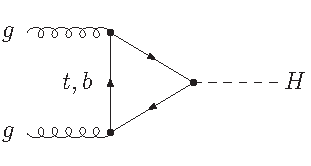
\includegraphics[width=\textwidth]{axodraw/ggF.pdf}
		\caption{Gluon-gluon fusion (ggF)}
		\label{fig:feyn:ggF}
	\end{subfigure}
	\hfill
	\begin{subfigure}[b]{0.4\textwidth}
		\centering
		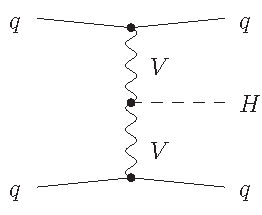
\includegraphics[width=0.75\textwidth]{axodraw/VBF.pdf}
		\caption{Vector boson fusion (VBF)}
		\label{fig:feyn:VBF}
	\end{subfigure}
	\hfill\null
	\\\bigskip
	\null\hfill
	\begin{subfigure}[b]{0.4\textwidth}
		\centering
		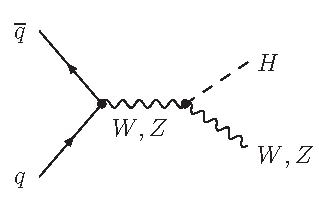
\includegraphics[width=0.8\textwidth]{axodraw/VH.pdf}
		\caption{Higgs-strahlung (\WH and \ZH)}
		\label{fig:feyn:VH}
	\end{subfigure}
	\hfill
	\begin{subfigure}[b]{0.4\textwidth}
		\centering
		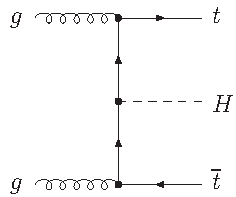
\includegraphics[width=0.625\textwidth]{axodraw/ttH.pdf}
		\caption{Top fusion (\ttH)}
		\label{fig:feyn:ttH}
	\end{subfigure}
	\hfill\null
	\caption{Examples of tree-level Feynman diagrams for the Higgs production processes relevant at the LHC.}
	\label{fig:feyn}
\end{figure}

The production cross sections at the LHC are shown in \Figure~\ref{fig:higgs_xs}. 
Whilst ggF clearly dominates these rare processes, it suffers from large 
experimental backgrounds. The four other modes feature additional final state particles 
which can aid identification. For example, VBF has two well-separated quarks with no 
colour exchange between them.

\begin{figure}
	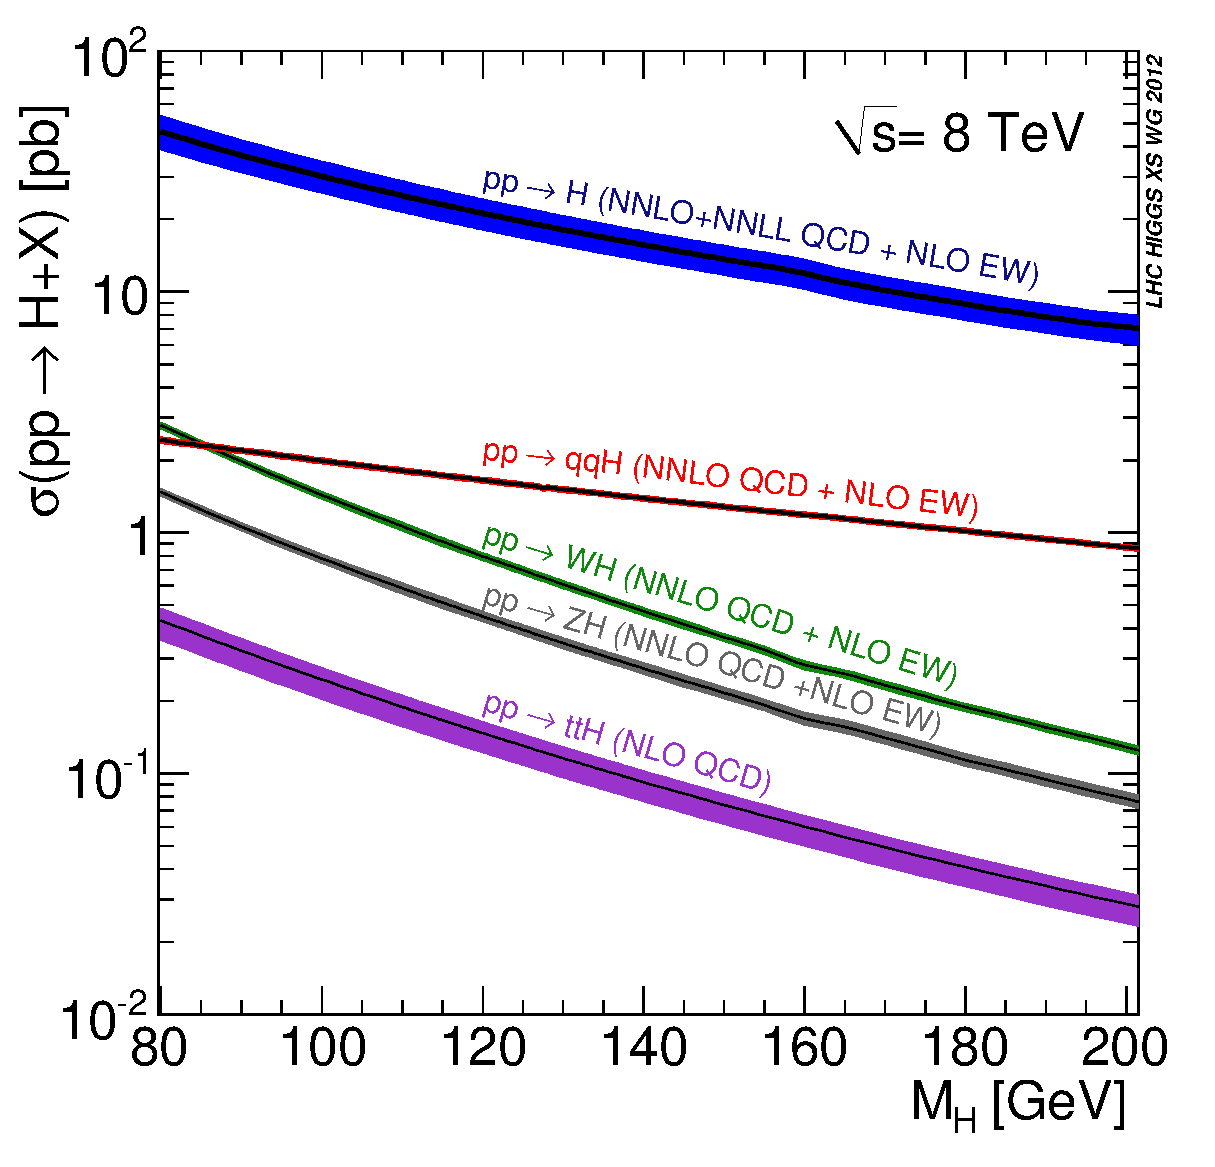
\includegraphics[width=0.48\textwidth]{tex/motivation/xs_lowrange}
	\hfill
	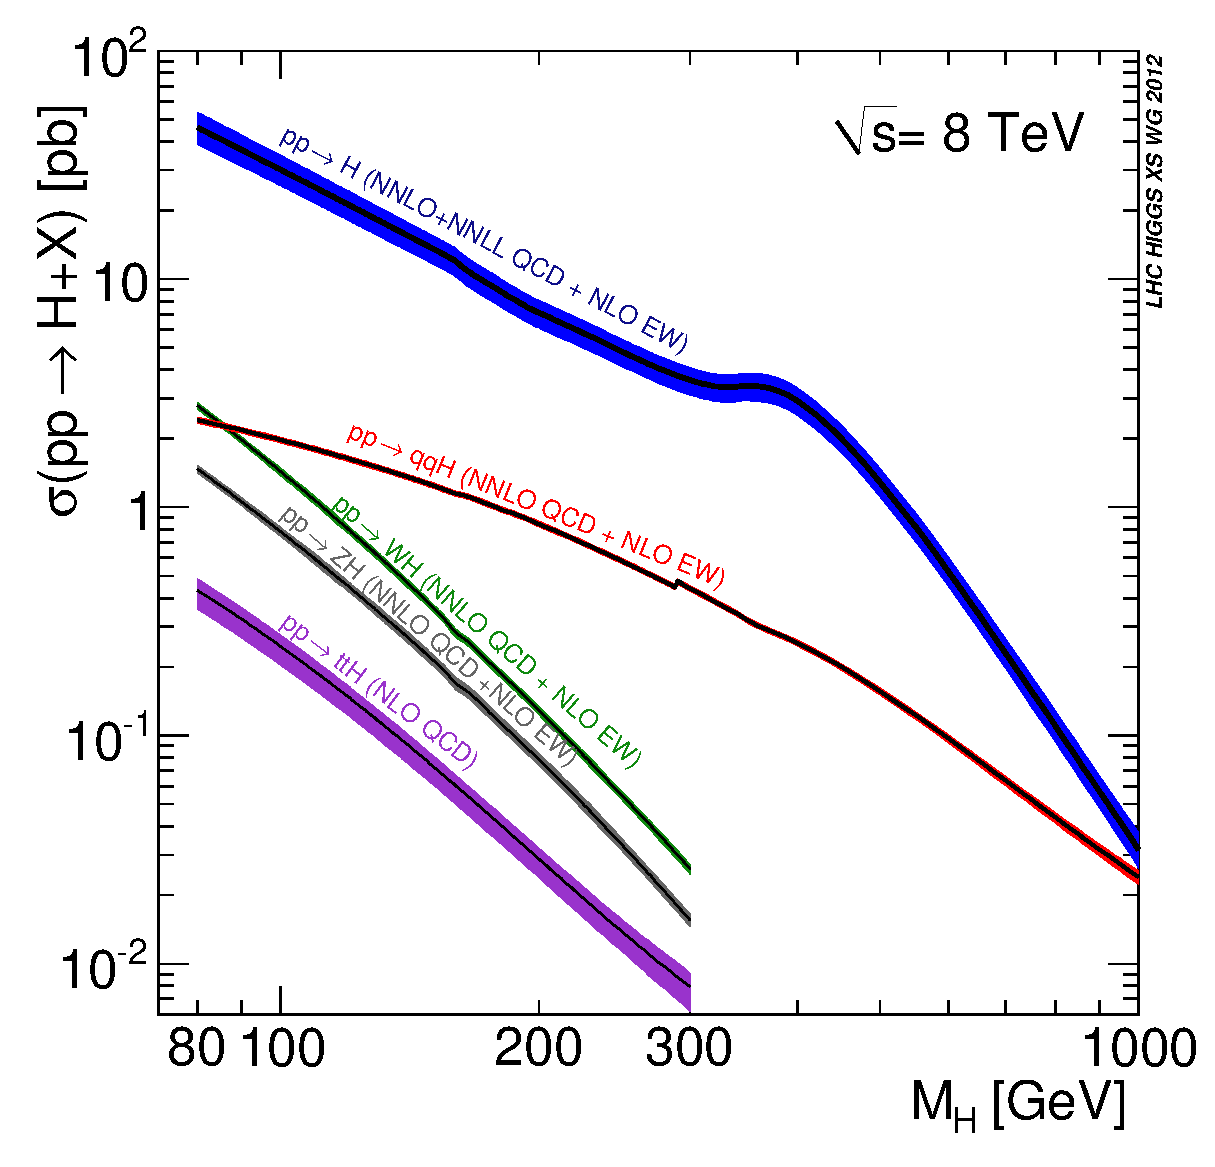
\includegraphics[width=0.48\textwidth]{tex/motivation/xs_fullrange}
	\caption{Higgs boson production cross sections versus mass at 
	\unit{$\sqrt{s} = 8$}{\TeV} for a low mass range (left) and an expanded mass range 
	(right) \cite{YR2}. Theoretical uncertainties are shown as bands. The production modes
	are ggF (blue), VBF (red), \WH (green), \ZH (grey) and \ttH (purple).}
	\label{fig:higgs_xs}
\end{figure}

Since the lifetime of the Higgs boson is very short, it is never directly observed in a 
detector. Therefore it is important to understand the BRs of its decays 
(\Figure~\ref{fig:higgs_br}). Na\"{i}vely, these are understood from the Higgs boson coupling to mass and the kinematic requirement $m_{\PHiggs} > m_X + m_Y$ for a decay
\HepProcess{\PHiggs \HepTo XY}. This is complicated by off-shell particles (\eg a low mass
Higgs boson may decay to \HepProcess{\PW \PW^{*}}). 
Also, the \HepProcess{\Pphoton \Pphoton}, \HepProcess{\PZ \Pphoton} and 
\HepProcess{\Pgluon \Pgluon} decay modes are different since they feature massless 
particles, and therefore proceed via loops of massive charged particles (electric charge 
for \HepProcess{\Pphoton \Pphoton} and \HepProcess{\PZ \Pphoton}, colour charge for 
\HepProcess{\Pgluon \Pgluon}).

Designing a sensitive experimental search strategy for the Higgs boson can be difficult. 
In decay channels featuring weak bosons, the subsequent decay of the \PW or \PZ boson must 
also be considered. These are more likely to decay to quarks than to leptons, but the 
former suffers from large backgrounds at hadron colliders. Similarly, the 
\HepProcess{\Pbottom \APbottom} decay has the largest BR for low \mH but suffers from 
huge backgrounds. The sensitivity can be improved by combining with a more distinguished 
production mode, such as \WH or \ZH, but this reduces the production cross section.

\begin{figure}
	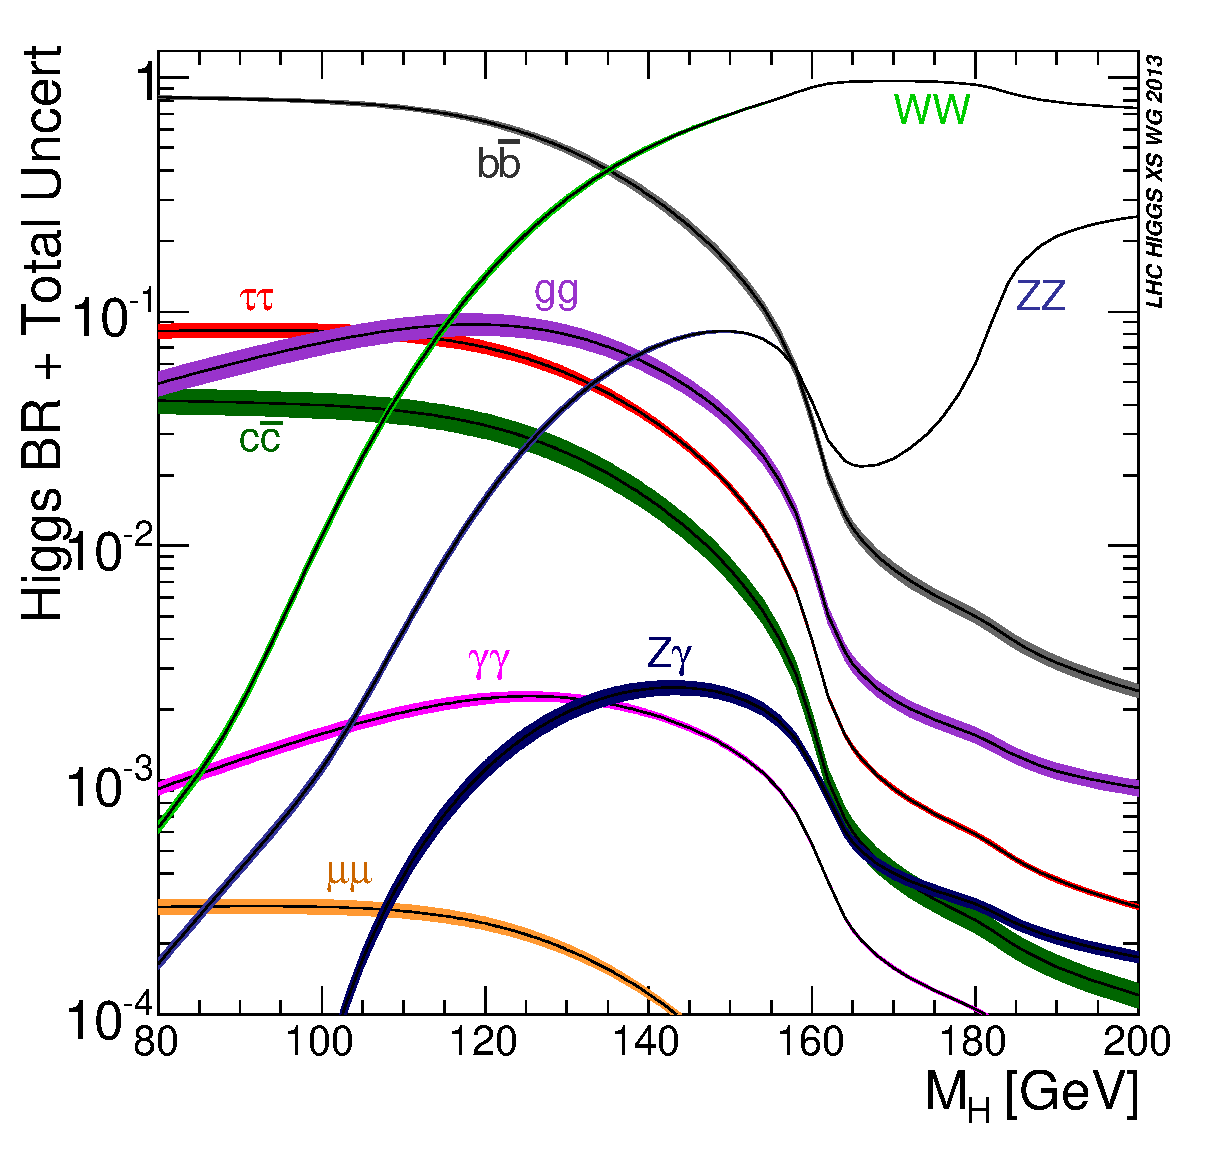
\includegraphics[width=0.48\textwidth]{tex/motivation/BR_lowrange}
	\hfill
	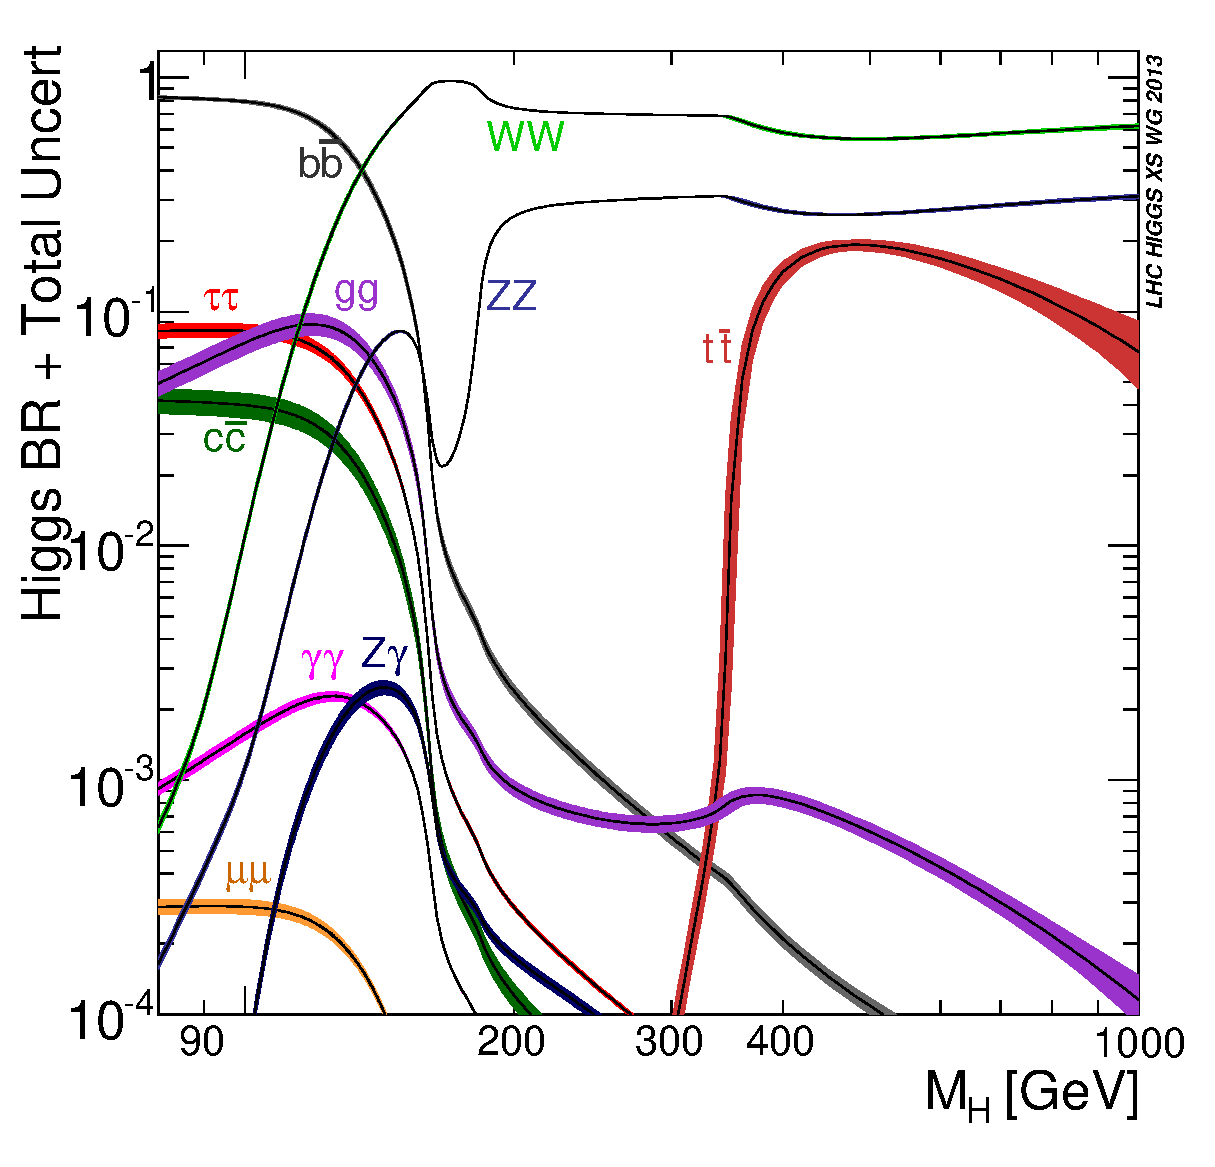
\includegraphics[width=0.48\textwidth]{tex/motivation/BR_fullrange}
	\caption{Branching ratios of Higgs boson decay versus mass for a low mass range (left) 
	and an expanded mass range (right) \cite{YR3}. Theoretical uncertainties are shown as 
	bands.}
	\label{fig:higgs_br}
\end{figure}

\section{Pre-LHC constraints on the Higgs boson mass}
	\label{sec:prior_constraints}
	%!TEX root = ../../thesis.tex

Neglecting Yukawa interactions, the EW sector of the SM contains several free 
parameters that must be experimentally determined: two couplings ($g$, $g'$) and two 
Higgs sector parameters ($\mu$, $\lambda$). Using relations in \Section~\ref{sec:ewsb}, 
it is advantageous to choose an alternative set of independent parameters more closely 
connected to experiment: \alphaEM, \mW, \mZ, \mH. Finding the Higgs boson and 
measuring its mass is therefore of fundamental importance to understanding the EW 
sector, and this was a primary goal of the LHC physics program.

Prior to the LHC, the value of \mH was constrained through direct searches at 
previous colliders, global fits of other electroweak observables and theoretical 
considerations.



\subsection{Direct searches}
\label{sec:prior_constraints:direct}

Although masses below \unit{4}{\GeV} were excluded from \PB, \PUpsilon and \PK meson 
decays \cite{PDG:1988}, the first meaningful searches for a Higgs boson were 
performed at LEP (CERN, Geneva), which ran from 1989 to 2000. This was a circular 
\epluseminus collider with a centre-of-mass (CM) energy tuned to the \PZ-pole and then 
later varied between 189 and \unit{209}{\GeV}. A combined search for \ZH was performed 
using a total integrated luminosity of \unit{2.5}{\invfb}, which excluded 
\unit{$\mH < 114.4$}{\GeV} at the 95\% confidence level (CL) \cite{LEP:2003}.

Further searches were performed at the Tevatron (FNAL, Illinois), which ran from 1987
to 2011. This was a circular \ppbar collider with CM energies of \unit{1.8}{\TeV}
and \unit{1.96}{\TeV}. In 2010, searches using a variety of production and decay modes 
were combined across experiments using a total integrated luminosity of up to
\unit{12.6}{\invfb}. Masses below \unit{109}{\GeV} and between 158 and \unit{175}{\GeV} 
were excluded at the 95\% CL \cite{Tevatron:2010}.

% \begin{figure}
% 	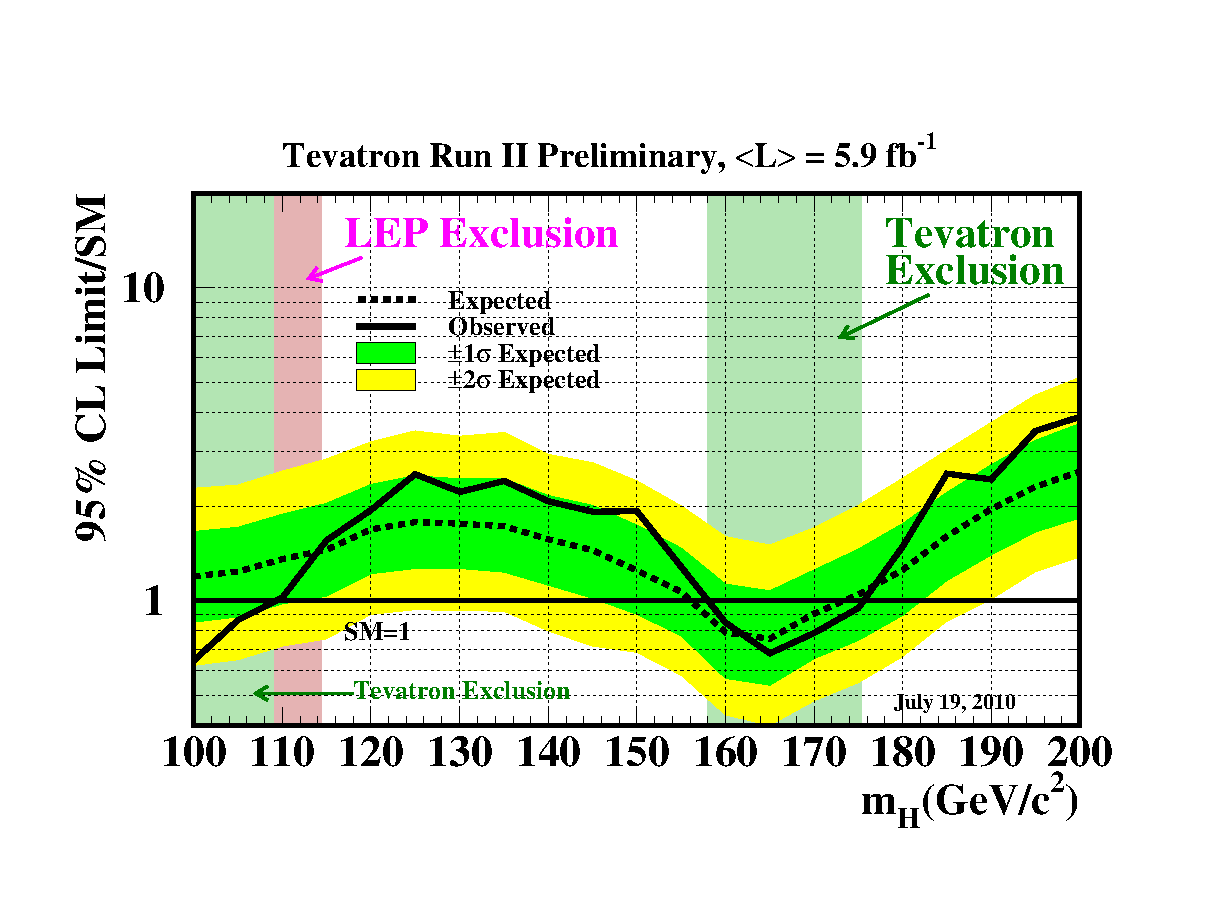
\includegraphics[width=\mediumfigwidth]{tex/motivation/tevatron_limit}
% 	\caption{Observed and expected 95\% \ac{CL} upper limits on the ratio to the \ac{SM} 
% 	cross section versus \mH, obtained through combination of multiple CDF and \dzero 
% 	analyses \cite{Tevatron:2010}. The analyses use datasets corresponding to integrated 
% 	luminosities up to \unit{5.9}{\invfb} at CDF and up to \unit{6.7}{\invfb} at \dzero.}
% 	\label{fig:existing_limits}
% \end{figure}



\subsection{Precision electroweak fits}
\label{sec:prior_constraints:ew_fits}

The SM predicts that many observables will depend upon \mH through loop corrections,
and it is therefore possible to infer \mH through precision EW measurements. Since 
the leading \mH dependence is logarithmic, the inferred constraints are weaker than those
used to predict the top mass (where the dependence is quadratic).

Performing a global fit of various electroweak measurements at the LEP, SLC and
Tevatron colliders (\eg \mW, \mZ, $m_{\Ptop}$), in July 2010 it was possible to exclude 
\mH $>$ \unit{158}{\GeV} at the 95\% CL \cite{Gfitter:2008}. However, the best fit 
value was excluded by direct searches, as shown in \Figure~\ref{fig:ewfit}.

\begin{figure}[t]
	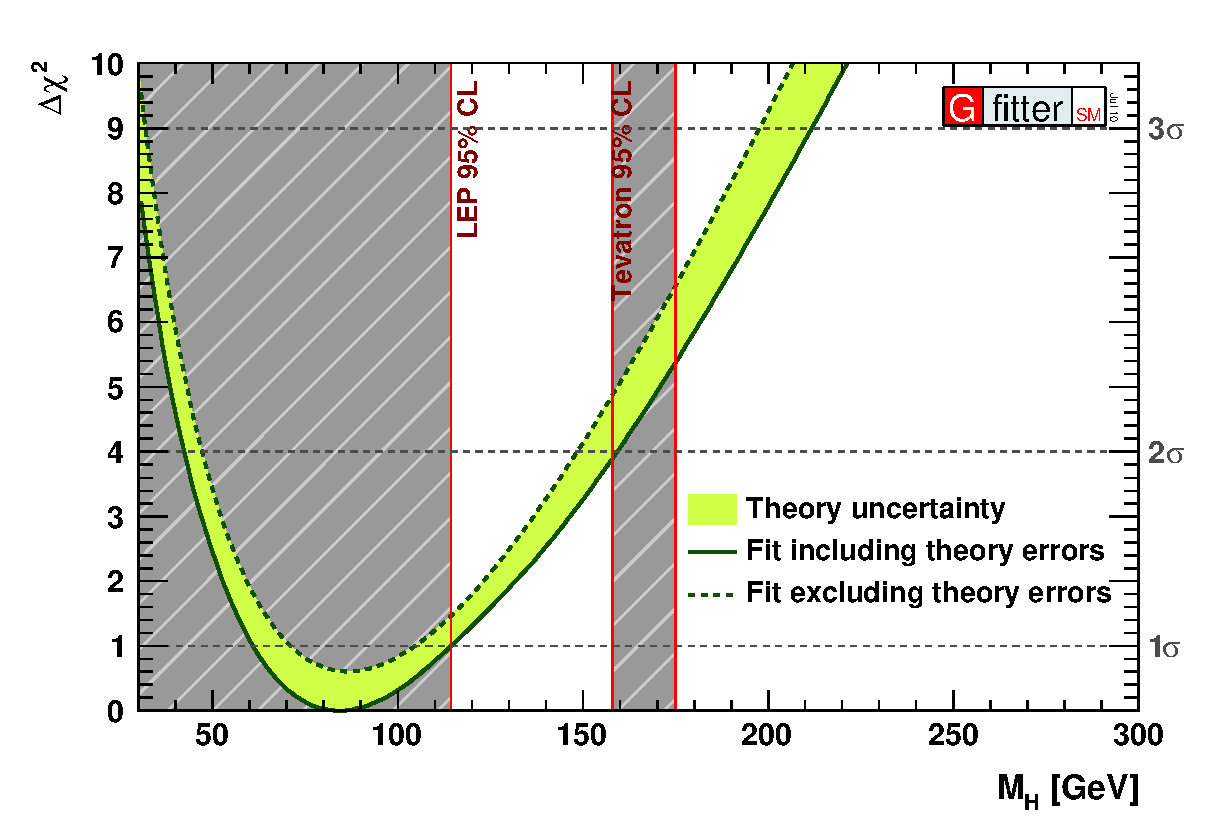
\includegraphics[width=0.495\textwidth]{tex/motivation/ewfit_nodirect}
	\hfill
	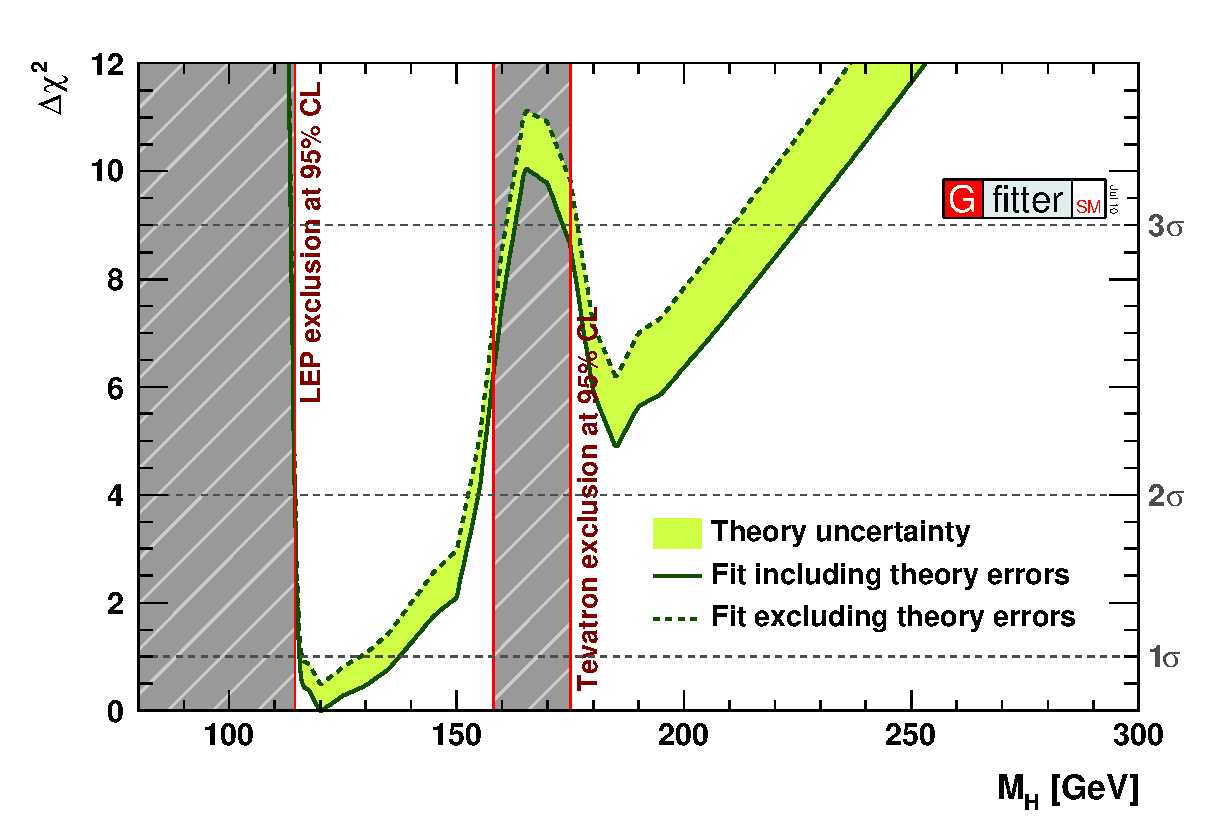
\includegraphics[width=0.495\textwidth]{tex/motivation/ewfit_withdirect}
	\caption{The observed $\Delta\chi^2 = \chi^2 - \chi^2_{\min}$ of electroweak fits 
	versus \mH, neglecting (left) and including (right) results from direct searches
	\cite{Gfitter:2008}. The exclusion limits from LEP and the Tevatron are also shown.
	These results were produced in July 2010. 
	With kind permission from Springer Science and Business Media.}
	\label{fig:ewfit}
\end{figure}

% \begin{figure}
% 	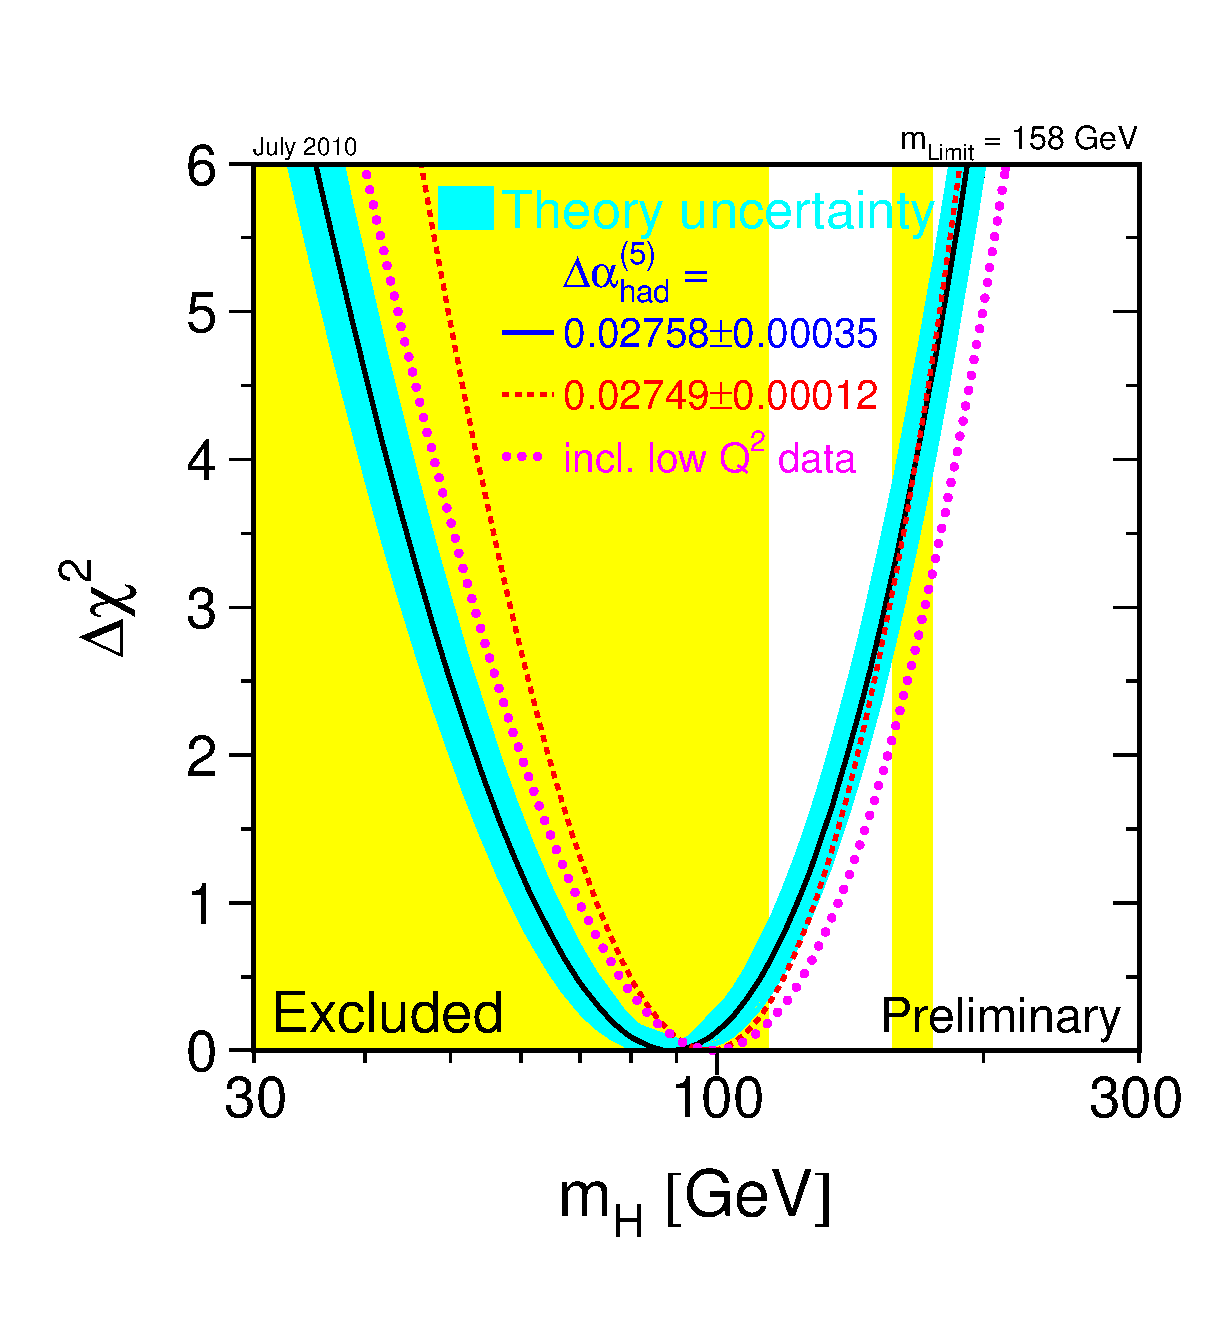
\includegraphics[width=\mediumfigwidth]{tex/motivation/ew_fit_chi2}
% 	\caption{The observed $\Delta\chi^2 = \chi^2 - \chi^2_{\min}$ of electroweak fits 
% 	versus \mH \cite{Grunewald:2010}. The line is fit using \PZ-pole data and direct 
% 	measurements of \mW, $\Gamma_{\PW}$ and $m_{\Ptop}$, and the band is an estimate of 
% 	the uncertainty due to missing higher order corrections. The dashed line uses an 
% 	alternative value of the hadronic vacuum polarisation to show the effect of 
% 	uncertainty in $\alpha(m_{\PZ}^2)$. The dotted line includes low-$Q^2$ experimental 
% 	data. The vertical bands show the 95\% \ac{CL} exclusion limits on \mH arising from 
% 	direct searches at the \ac{LEP} and the Tevatron.}
% 	\label{fig:ewfit}
% \end{figure}



\subsection{Theoretical constraints}
\label{sec:prior_constraints:theory}

Like all coupling constants in a renormalisable theory (see 
\Section~\ref{sec:qcd:renormalisation}), the Higgs quartic coupling $\lambda$ `runs' with 
energy scale $\Lambda$, as described by the renormalisation group equations (RGEs). The 
running is characterised by the $\beta$-function:
\begin{equation*}
	\beta_{\lambda} = \frac{\partial \lambda}{\partial \log\Lambda} \,.
\end{equation*}

For high \mH, self-couplings dominate $\beta_{\lambda}$, which have a
positive contribution. Therefore $\lambda$ increases with the scale, and above some 
critical scale $\Lambda_{\text{c}}$ the EW theory is no longer perturbative. Thus we 
would either expect to observe non-perturbative behaviour at scales 
\about$\Lambda_{\text{c}}$ or new physics at a scale $<\Lambda_{\text{c}}$ that 
circumvents this issue. Larger values of \mH lead to lower values of $\Lambda_{\text{c}}$ 
and are therefore disfavoured (blue line in \Figure~\ref{fig:theory_constraints}). 
Requiring perturbativity up to the reduced Planck scale of 
\unit{$\bar{\Lambda}_{\text{P}}~\about~10^{18}$}{\GeV} (where we expect new physics 
describing gravity) places an upper bound on \mH of \unit{175}{\GeV} \cite{Ellis:2009}.

For small \mH, top loops dominate $\beta_{\lambda}$, which have a negative 
contribution. Therefore $\lambda$ decreases as the scale increases, and above some 
critical scale $\Lambda_{\text{c}}$ the coupling becomes negative. Then the EW 
vacuum is simply a local minimum and it is possible for the Universe to collapse through
quantum tunnelling into the more stable vacuum state (yellow band in 
\Figure~\ref{fig:theory_constraints}). Requiring vacuum stability up to 
$\bar{\Lambda}_{\text{P}}$ places a lower bound on \mH of \unit{129}{\GeV} 
\cite{Ellis:2009}. 
It is also possible to consider a metastable Universe whose expected lifetime is longer 
than its age. Accounting for thermal fluctuations up to temperatures 
\about$\bar{\Lambda}_{\text{P}}$, the EW vacuum has a lifetime longer than the age 
of the Universe if \mH $>$ \unit{122}{\GeV} (pale blue band in 
\Figure~\ref{fig:theory_constraints}) \cite{Ellis:2009}. These bounds are rather 
sensitive to the top mass, which is 
$m_{\Ptop} = \statsyst{173.34}{0.27}{0.71}~\GeV$ \cite{TopMass}.

\begin{figure}[t]
	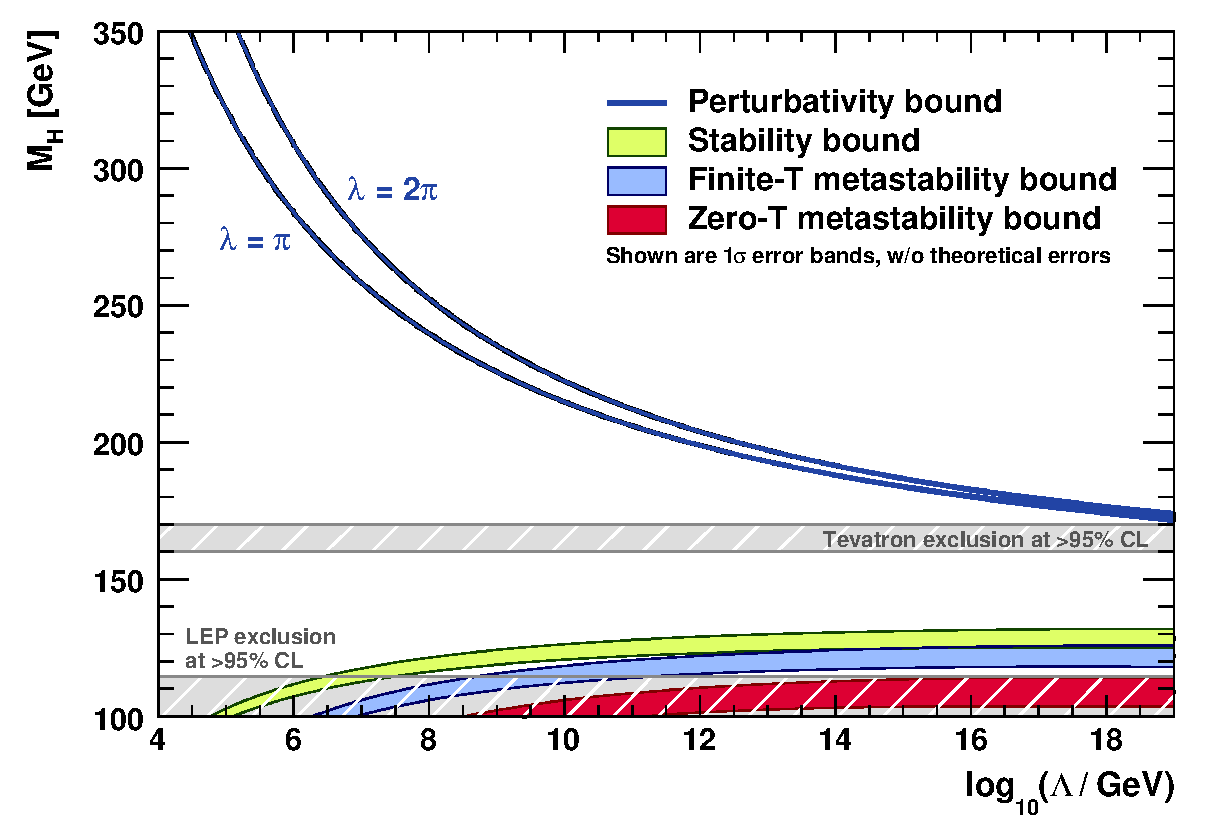
\includegraphics[width=\mediumfigwidth]{tex/motivation/theory_constraints}
	\caption{The scale $\Lambda$ at which the Higgs quartic coupling becomes 
	non-perturbative (blue lines) or an instability in the EW vacuum appears
	(yellow band) \cite{Ellis:2009}. The two blue lines represent different degrees of 
	non-perturbativity (lower line corresponds to a two-loop correction of 25\%, upper 
	line is 50\%), and their difference is indicative of the theoretical uncertainty in 
	this bound. The blue and red bands are bounds for a metastable Universe including and
	neglecting thermal fluctuations respectively. Reprinted from Physics Letters~B \textbf{679}, 4,
	J.~Ellis, J.~R.~Espinosa, G.~F.~Giudice, A.~Hoecker and A.~Riotto, \textit{The Probable 
	Fate of the Standard Model}, 369--375, Copyright (2009), with permission from Elsevier.}
	\label{fig:theory_constraints}
\end{figure}


\bibliographystyle{thesis}
\bibliography{theory,pheno,mc,experiment}
